\documentclass[manuscript]{clv2025}

\jvol{vv}
\jnum{nn}
\jyear{2026}
\jinfo{}
\renewcommand{\footmark}{}
\dochead{Position Paper}

%% Choose your variant of English
\usepackage[american]{babel}

%% Required packages
\usepackage{natbib}
    \bibliographystyle{compling}
\usepackage{mathtools}
\usepackage{booktabs}
\usepackage{tikz}
\usetikzlibrary{shapes.geometric, arrows.meta, positioning, fit, calc}
\usepackage{multirow}
\usepackage{graphicx}
\usepackage{xcolor}
\usepackage{amsmath}
\usepackage{amssymb}

\usepackage{tabularx}
\usepackage{array}
\hypersetup{hidelinks}

\makeatletter
\renewcommand{\appendixsection}[1]{%
   \refstepcounter{section}%
   \setcounter{subsection}{0}%
   \setcounter{subsubsection}{0}%
   \setcounter{table}{0}%
   \setcounter{figure}{0}%
   \setcounter{equation}{0}%
   \section*{Appendix \Alph{section}: #1}%
}
\makeatother



%% Drafting helpers (remove for camera-ready)
%% ------------------------------------------------------------
% (draft helper macros removed for submission)

%% ------------------------------------------------------------
%% Vocabulary (normalize throughout paper)
%% ------------------------------------------------------------
% \newcommand{\CI}{\textsc{CI}} % creative intent -- removed from the framework vocabulary
\newcommand{\TC}{\textsc{TC}} % truth contract
\newcommand{\TCs}{\textsc{TC}s} % truth contract (plural)
\newcommand{\LD}{\textsc{LD}} % licensed divergence
\newcommand{\Hall}{\textsc{H}} % hallucination (TR-violating)
\newcommand{\Faith}{\textsc{F}} % faithfulness
\newcommand{\Acc}{\textsc{A}} % accuracy/factuality

%% ------------------------------------------------------------
%% Palette and TikZ styles for the claim-annotation decision tree (Fig.)
%% ------------------------------------------------------------
\definecolor{clrH}  {RGB}{155, 18, 18}   % hallucination
\definecolor{clrPD} {RGB}{ 22, 98, 48}   % licensed divergence
\definecolor{clrOK} {RGB}{ 50, 50, 50}   % ok / neither
\definecolor{clrUV} {RGB}{160, 95,  8}   % unverifiable
\definecolor{clrKw} {RGB}{ 22, 52,125}   % spine / keyword
\definecolor{clrPh} {RGB}{ 38, 38, 88}   % header
\definecolor{phbg}  {RGB}{228,232,246}   % header background
\definecolor{decbg} {RGB}{245,247,254}   % decision node bg
\definecolor{decbdr}{RGB}{125,150,198}   % decision node border
\tikzset{
  inpnode/.style={rectangle, rounded corners=5pt, draw=gray!50, fill=gray!9,
    font=\small\itshape, text width=5.2cm, align=center, inner xsep=6pt, inner ysep=5pt},
  decnode/.style={rectangle, rounded corners=3pt, draw=decbdr, fill=decbg,
    font=\small, text width=5.2cm, align=center, inner xsep=6pt, inner ysep=4pt},
  lSV/.style={rectangle, rounded corners=3pt, draw=clrOK!50, fill=clrOK!7,
    font=\small\bfseries\sffamily, text=clrOK!75, inner xsep=7pt, inner ysep=4pt},
  lOK/.style={rectangle, rounded corners=3pt, draw=clrOK, fill=clrOK!12,
    font=\small\bfseries\sffamily, text=clrOK, inner xsep=7pt, inner ysep=4pt},
  lUV/.style={rectangle, rounded corners=3pt, draw=clrUV, fill=clrUV!10,
    font=\small\bfseries\sffamily, text=clrUV, inner xsep=7pt, inner ysep=4pt},
  lH/.style={rectangle, rounded corners=3pt, draw=clrH, fill=clrH!9,
    font=\small\bfseries\sffamily, text=clrH, inner xsep=7pt, inner ysep=4pt},
  lPD/.style={rectangle, rounded corners=3pt, draw=clrPD, fill=clrPD!9,
    font=\small\bfseries\sffamily, text=clrPD, inner xsep=7pt, inner ysep=4pt},
  lNE/.style={rectangle, rounded corners=3pt, draw=clrOK!40, fill=clrOK!6,
    font=\small\bfseries\sffamily, text=clrOK!65, inner xsep=7pt, inner ysep=4pt},
  arr/.style={-{Stealth[length=4.8pt,width=3.4pt]}, thick, color=gray!58!black},
  spinelbl/.style={font=\scriptsize\sffamily\bfseries, text=clrKw!85, fill=white,
    inner sep=1.5pt, rounded corners=1pt},
  exitlbl/.style={font=\scriptsize\sffamily, text=gray!68!black, fill=white,
    inner sep=1.5pt, rounded corners=1pt},
  annot/.style={font=\scriptsize\itshape, text=gray!60},
}

%% ------------------------------------------------------------
%% tcolorbox cards for the thesis-at-a-glance table (Table 1)
%% ------------------------------------------------------------
\usepackage[most]{tcolorbox}
\definecolor{cardStrict}{HTML}{2F5597}
\definecolor{cardStyle} {HTML}{2E7D6B}
\definecolor{cardFlag}  {HTML}{6A4C93}
\definecolor{cardIdea}  {HTML}{B45F06}
\newcommand{\vbadge}[2]{\tcbox[on line, colback=#1, colframe=#1, boxrule=0pt, arc=2pt,
  left=3pt, right=3pt, top=0.4pt, bottom=0.4pt, boxsep=0pt]{\scriptsize\bfseries\textcolor{white}{#2}}}
\newcommand{\bH}{\vbadge{clrH}{H}}
\newcommand{\bPD}{\vbadge{clrPD}{LD}}
\newcommand{\bNE}{\vbadge{clrOK}{neither}}
\newcommand{\bIP}{\vbadge{clrUV}{insuff.\ LD}}
\newcommand{\skb}[2]{\tcbox[on line, colback=#1!12, colframe=#1!55!black, boxrule=0.3pt, arc=2pt,
  left=3pt, right=3pt, top=0.4pt, bottom=0.4pt, boxsep=0pt]{\scriptsize\bfseries #2}}
\tcbset{regcard/.style={enhanced, width=\linewidth, boxrule=0.4pt, arc=3pt,
  left=7pt, right=7pt, top=3pt, bottom=4pt, before skip=3pt, after skip=3pt,
  fonttitle=\bfseries\small, coltitle=black,
  attach boxed title to top left={xshift=7pt, yshift=-2.2mm},
  boxed title style={boxrule=0pt, arc=2pt, left=5pt, right=5pt, top=1.5pt, bottom=1.5pt}}}

\title{Hallucination Is Relative: A Position on Truth-Contract-Aware Evaluation of LLM Divergence}

\runningtitle{Hallucination Is Relative}
\runningauthor{Carlesso et al.}

\author{Mathis Carlesso$^{1,2}$, Martino Lovisetto$^{2}$, Elöd Egyed-Zsigmond$^{1}$, Pierre-Yves Genest$^{2}$, Stefan Duffner$^{1}$}

\affilblock{
    \affil{INSA Lyon, CNRS, LIRIS, UMR5205, Université Claude Bernard Lyon 1, 69621 Villeurbanne, France\\\quad \email{mathis.carlesso@insa-lyon.fr}}
    \affil{Alteca, 69100 Villeurbanne, France}
}


\begin{document}
\maketitle

\begin{abstract}
Large language model hallucination is often treated as unsupported content.
This view ignores what the prompt permits.
The same unsupported claim can be harmful in a medical answer, acceptable in fiction, or useful when clearly presented as a hypothesis.
We therefore propose a prompt-level \emph{truth contract}, $\TC(p)=(O_p,\sigma_p,\kappa_p)$.
The oracle $O$ specifies the evidence against which claims are evaluated.
The form license $\sigma$ specifies how freely the answer may vary in style.
The content license $\kappa$ specifies whether new content may be added, where it is allowed, and how it must be presented.
Under this framework, hallucination (\Hall) is a contract violation.
Licensed divergence (\LD) is a departure from oracle support that falls within the licensed scope and uses the required stance; its usefulness is evaluated separately.
We support this position with a scoping audit of forty hallucination and creativity evaluation resources and four worked cases.
The audit suggests that existing protocols often specify an oracle but rarely represent form and content licenses as explicit scoring variables.
The cases show that the same claim can be \Hall\ under one contract and \LD\ under another.
We conclude with a research agenda for contract-aware benchmarks, claim-level annotation, and mitigation methods that reduce \Hall\ without suppressing \LD.
\end{abstract}


\section{Introduction: The Creativity--Hallucination Paradox}\label{sec:intro}

Large language models (LLMs) sometimes state things that are not true.
The community calls these errors \emph{hallucinations}: the model produces fluent, confident text that is not supported by evidence or contradicts known facts \citep{ji_survey_2023, huang_survey_2025}.
Hallucination is widely regarded as the central reliability barrier for deploying LLMs in high-stakes settings such as medicine, law, and education \citep{lin_truthfulqa_2022}.
A large body of work consequently aims to detect, measure, and reduce it \citep{li_halueval_2023, wei_measuring_2024, thorne_fever_2018}.

This effort hides a paradox.
When users ask an LLM to write fiction, brainstorm, or propose creative solutions, they want the model to go beyond established facts. Punishing every unsupported statement would suppress exactly the outputs these users ask for \citep{franceschelli_creativity_2024, hou_creativityprism_2025, rick_supermind_2023}.
A brainstorming tool that only repeats ideas that already exist is useless; a medical assistant that invents diagnoses is dangerous.
The difference lies not in the text itself, but in what the prompt asked for.

\paragraph{The diagnostic gap.}
Current evaluation practice does not capture this difference.
Hallucination benchmarks treat any unsupported content as a defect to minimize \citep{bang_hallulens_2025}, whereas creativity benchmarks treat novelty as a virtue to maximize, often without checking factual grounding \citep{hou_creativityprism_2025, acar_creativity_2019}.
Neither tradition conditions its scores on what the user's prompt actually licenses.
As a result, one output can be scored as a serious failure by one tradition and a creative success by another, depending on which protocol is applied rather than on whether the divergence was appropriate.

Even the closest recent work does not model the contract.
Intent-aware evaluation checks whether a response covers the query's constraints, but it has neither $O$ nor $\kappa$ \citep{hao_faithqa_2025}. The closest work splits hallucinations into ``intelligent'' and ``defective'', but it derives the label from the output, not from the prompt: the same output always keeps the same label, whatever the prompt asked for \citep{yang_hicbench_2025}.
Section~\ref{sec:sota} examines both.
Neither makes $(O,\sigma,\kappa)$ a scored variable, and that omission is the gap we identify.

Better detectors alone do not solve this. The missing variable is not evidential support but license: did the task allow the model to go beyond the evidence?
Recent theoretical arguments moreover suggest that unsupported generation will not disappear under broad task distributions: arguments based on incompleteness and undecidability \citep{banerjee_llms_2024, xu_hallucination_2024} suggest that some level of error will remain, no matter how well the model is trained.
Yet the same generative mechanism also produces the novel hypotheses and creative combinations that users request in open-ended tasks \citep{sun_hallucinating_2024, he_shakespearean_2025}.
The goal, therefore, cannot be to eliminate divergence, but to judge it against what the task permits.

\paragraph{Our thesis.}
Hallucination is not a context-free property of a claim.
It is a verdict relative to the prompt's \emph{truth contract}, $\TC(p)=(O_p,\sigma_p,\kappa_p)$.
The oracle $O$ defines the relevant standard of support.
The form license $\sigma$ defines how freely the answer may vary in style.
The content license $\kappa$ defines whether new content is allowed, its scope, and the stance (asserted as fact, or marked as a hypothesis) required when presenting it.
Under a strict contract (for example, ``summarize this document accurately''), an unsupported claim is a hallucination (\Hall).
Under a permissive contract (for example, ``write fiction''), the same claim may be \emph{licensed divergence} (\LD).
The contract does not change what is true.
It changes whether the model's departure violates the task.
Figure~\ref{fig:flip} shows this on one example.
This is also what separates \TC\ from context-faithfulness: faithfulness asks only whether an output stays within its evidence, and has no analogue of $\kappa$, the explicit license to go beyond it.
Table~\ref{tab:thesis-at-a-glance} (Section~\ref{sec:framework}) previews the thesis on representative prompts.

% ============================================================
% One-example summary of the thesis (same claim, two contracts)
% ============================================================
\begin{figure}[t]
\centering
\resizebox{0.92\linewidth}{!}{%
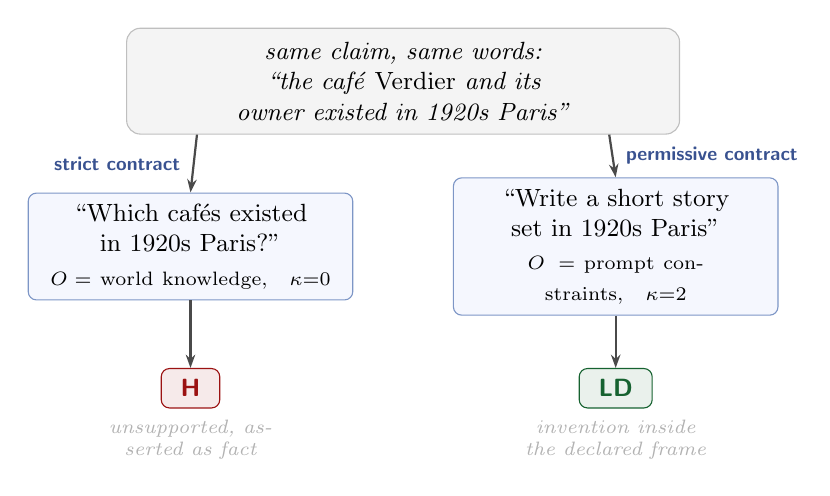
\begin{tikzpicture}[x=1cm, y=1cm]
\node[inpnode, text width=6.6cm] (claim) at (0,0)
  {same claim, same words:\\``the caf\'e \emph{Verdier} and its owner existed in 1920s Paris''};
\node[decnode, text width=3.7cm] (p1) at (-2.7,-2.1)
  {``Which caf\'es existed in 1920s Paris?''\\[1pt]{\scriptsize $O=$ world knowledge,\quad$\kappa{=}0$}};
\node[decnode, text width=3.7cm] (p2) at (2.7,-2.1)
  {``Write a short story set in 1920s Paris''\\[1pt]{\scriptsize $O=$ prompt constraints,\quad$\kappa{=}2$}};
\node[lH]  (v1) at (-2.7,-3.9) {\textsf{H}};
\node[lPD] (v2) at (2.7,-3.9) {\textsf{LD}};
\node[annot, text width=3.6cm, align=center] at (-2.7,-4.55) {unsupported, asserted as fact};
\node[annot, text width=3.6cm, align=center] at (2.7,-4.55) {invention inside the declared frame};
\draw[arr] (claim.south west) ++(0.9,0) -- node[spinelbl, left=3pt] {strict contract} (p1.north);
\draw[arr] (claim.south east) ++(-0.9,0) -- node[spinelbl, right=3pt] {permissive contract} (p2.north);
\draw[arr] (p1) -- (v1);
\draw[arr] (p2) -- (v2);
\end{tikzpicture}}
\caption{\textbf{The thesis on one example.}
The same claim receives two different verdicts: hallucination (\Hall) under a strict contract, licensed divergence (\LD) under a permissive one.
The contract, not the text, decides the verdict (Case~B, Section~\ref{sec:worked}).}
\label{fig:flip}
\end{figure}

\paragraph{How we support the position.}
We support this position with two analyses.
First, we conduct a scoping audit of forty hallucination and creativity evaluation resources.
The audit asks whether each protocol explicitly represents the oracle, the form license, and the content license as scoring variables (Section~\ref{sec:sota}).
Second, we apply our claim-level rule to four worked cases (Section~\ref{sec:worked}).
The audit identifies a protocol-level omission; the cases show why this omission can change a verdict.
These analyses establish the conceptual gap, but they do not measure its prevalence.
A controlled contract-aware study is therefore left to future work.

\paragraph{Contributions.}
This position paper makes three contributions.
\emph{First} (conceptual), we introduce $\TC(p)=(O_p,\sigma_p,\kappa_p)$ and a minimal vocabulary (\TC, \LD, \Hall) that makes explicit what the prompt licenses.
The vocabulary separates the two components that bear on truth (the oracle $O$ and the content license $\kappa$) from the form license $\sigma$, which governs form and conditions measurement validity (Section~\ref{sec:framework}).
\emph{Second} (diagnostic), we show that hallucination and creativity evaluation share a blind spot (neither conditions its scores on the truth contract), and we demonstrate it concretely by a scoping audit of existing benchmarks and by applying the labeling rule to worked cases (Sections~\ref{sec:sota}~and~\ref{sec:worked}).
\emph{Third} (programmatic), we outline a research agenda for contract-aware benchmarks that score \Hall\ and \LD\ separately under explicit oracle and license annotations (Section~\ref{sec:agenda}).


\section{Terminology and Conceptual Framework}\label{sec:framework}

\paragraph{Motivation.}
The literature uses the word \emph{hallucination} broadly, but not consistently.
Surveys commonly group together factuality errors against world knowledge and faithfulness errors against a provided source, sometimes adding axes such as intrinsic versus extrinsic causes and different granularities \citep{ji_survey_2023, huang_survey_2025}.
Benchmarking work further argues that hallucination is often confused with factuality and that any verdict depends on the chosen oracle and on evaluator reliability \citep{bang_hallulens_2025}.
To reason about creativity--hallucination trade-offs, we settle on a minimal vocabulary that makes the prompt's \emph{truth contract} explicit.
Throughout, we separate \emph{prompt-level} variables (what the user requests) from \emph{output-level} properties (what the model produces), and adopt a \emph{claim-level} unit of analysis because evaluations vary by granularity.

The idea that speakers operate under shared expectations about truthfulness is much older than LLM evaluation.
Grice's maxim of quality makes truthfulness a default norm of cooperative conversation \citep{grice_logic_1975}, and interlocutors track what counts as established through common ground \citep{clark_using_1996, stalnaker_assertion_1978}.
The truth contract borrows this insight but makes it narrower. Gricean norms are implicit and global. $\TC(p)$ instead selects only the truth-related expectations, for one prompt at a time, in a form explicit enough to annotate and score.

\textbf{Truth contract (\TC; prompt-level contract).}
A task-specific contract $\TC(p)=(O_p,\sigma_p,\kappa_p)$ that specifies the standard of support (the oracle $O$), the form license ($\sigma$), and the content license ($\kappa$): what must be \emph{grounded}, how freely the \emph{form} may vary, and what may be \emph{invented}.
We write $O_p$, $\sigma_p$, and $\kappa_p$ for the components of $\TC(p)$, and drop the subscript $p$ when the prompt is clear from context.
\TC\ is needed because both the definition of ``hallucination'' and the evaluation oracle shift across settings \citep{bang_hallulens_2025}.
We treat $\TC(p)$ as an \emph{idealization}: in deployment the contract is shaped not only by the visible prompt but also by system instructions, domain conventions, and user expectations, and an ambiguous prompt may not determine it fully.
Inferring \TC\ under such ambiguity is itself an open problem (Section~\ref{sec:agenda}); we nonetheless locate the contract at the prompt because that is where evaluation can render it explicit and auditable.

\textbf{Content oracle ($O$).}
The standard of support against which truth-conditional claims are checked: a source document, a retrieval set, a database, world knowledge, or user-provided facts.
The same claim can be supported by one oracle and unsupported by another, so $O$ must be specified rather than assumed \citep{bang_hallulens_2025, ji_survey_2023}.

\textbf{Form license ($\sigma$).}
How freely the \emph{form} of the output may vary while preserving its propositions.
This axis is studied independently of content.
Style is not a single variable but a bundle of co-varying dimensions \citep{kang_style_2021}; it can be transferred while meaning is held fixed \citep{jin_deep_2022}, and the dual operation (moving facts across a fixed style) is equally well defined \citep{balepur_text_2023}.
Figurative devices such as metaphor and hyperbole change the form of a claim while leaving its truth conditions intact \citep{badathala_match_2023}.
Foregrounding, the long-standing notion that stylistically marked language (language that draws deliberate attention to its own form, for example through imagery or unusual phrasing) stands out against an unmarked, plain background \citep{leech_short_style_1981}, is reliably recognized by readers \citep{vanpeer_stylistics_2020}.
This is what lets a graded $\sigma$ be annotated rather than guessed, and established formality datasets and style-transfer metrics make the axis operationally measurable \citep{pavlick_empirical_2016, rao_dear_2018, briakou_evaluating_2021}.
For now we treat $\sigma$ as a coarse ``low''/``high'' distinction: low is literal, neutral form (no marked figures or authorial voice); high is strongly marked form (sustained imagery, salient voice).
We keep this scale binary deliberately. Defining a finer, validated scale for the form license --- in particular, deciding where the middle level lies --- requires ongoing work in stylistics; we therefore defer a graded $\sigma$ to future work (Section~\ref{sec:agenda}).
By construction, $\sigma$ licenses variation in form only: a metaphor that preserves the underlying proposition introduces no new truth-conditional content.
Two consequences determine $\sigma$'s role in the framework.
First, $\sigma$ is independent of truth.
Since it neither adds nor removes a proposition, it cannot by itself make a claim \Hall\ or \LD.
Varying it leaves both faithfulness (\Faith) and accuracy (\Acc) unchanged in principle: those verdicts turn only on $O$ and $\kappa$, the two components that bear on content.
Second, $\sigma$ still matters for measurement. When the form license is high, an automatic verifier may misread stylistic form as unsupported content. A contract that does not specify $\sigma$ therefore cannot guarantee that the \Hall\ count is valid. In short, $\sigma$ is not a third verdict axis: it is the dimension that must not distort the measurement of the other two (Section~\ref{sec:agenda}). When the requested form itself is not delivered, that is an instruction-following failure, measured separately, not a breach of the truth contract.

\textbf{Content license ($\kappa$).}
Whether new truth-conditional content may be introduced, within what scope, and with what stance.
We use three levels: $\kappa{=}0$, no invention (every truth-conditional claim must be supported by $O$); $\kappa{=}1$, flagged speculation (hypotheses and extrapolations are permitted provided they are marked as such); $\kappa{=}2$, free invention within a declared frame (fiction, ideation), bound by coherence and user-provided facts rather than by $O$.
Theoretically, $\kappa$ reflects the kind of speech act the prompt licenses.
At $\kappa{=}0$ the model must make genuine assertions, committing to the truth of what it adds to the common ground \citep{stalnaker_assertion_1978}.
A declared fictional frame ($\kappa{=}2$) licenses what \citet{searle_logical_1975} calls pretended assertions: utterances with the form of assertion but without the commitment to truth.
$\kappa{=}1$ sits in between and admits assertions explicitly marked as provisional.
The two permissions are independent: many real prompts request creative style without factual invention (for example, ``explain photosynthesis like a poet''), so $\sigma$ is high while $\kappa{=}0$, and figurative language is welcome but fabricated claims are not \citep{franceschelli_creativity_2024}.
Throughout, we write $\sigma$ ``low''/``high'' for the bottom/top of its scale, and refer to $\kappa$ by its level ($0$, $1$, or $2$).

\paragraph{What the contract is not.}
$(O,\sigma,\kappa)$ is not a relabeling of grounding, style, or task type.
$O$ determines what counts as support but cannot say whether going beyond the evidence is licensed.
$\sigma$ governs form but cannot license new truth-conditional content.
A task label is too coarse because the same task can pair a high form license with $\kappa{=}0$, or neutral form with $\kappa{>}0$.
$\kappa$ is the one component that nothing else can replace: it determines whether unsupported content is an error, a flagged hypothesis, or invention inside a declared frame.
The contract is also not a relabeling of user intent.
Intent describes what the user wants; the truth contract specifies which claims require support, which departures are allowed, and how those departures must be presented.
Unlike a general pragmatic principle, it defines variables that can be annotated and scored.

\textbf{Faithfulness (\Faith; output-level).}
Whether the output is \emph{supported by the provided evidence} (documents, retrieved passages, tables), without introducing unsupported details.
This is the central failure mode in grounded generation and summarization, where fluent outputs can exceed source support \citep{maynez_faithfulness_2020, kryscinski_evaluating_2020}.

\textbf{Accuracy / factuality (\Acc; output-level).}
Whether the claims that must be true under \TC\ are actually supported by an appropriate external source (for example, references, gold labels, or world knowledge).
This corresponds to question answering (QA) and fact-checking evaluation.

\textbf{Hallucination (\Hall; claim-level).}
As we define it, a hallucination is unlicensed divergence, a breach of the truth contract: the model presents a claim \emph{as grounded/true} where \TC\ requires truth or evidence, but the claim is unsupported (\Faith) and/or incorrect (\Acc).
This unifies faithfulness and factuality failures while making the oracle explicit \citep{maynez_faithfulness_2020, bang_hallulens_2025}.

\textbf{Licensed divergence (\LD; claim-level).}
Content that would count as hallucination under a strict factual standard, but that the prompt's truth contract permits.
A claim is \LD\ when two conditions hold: it is \emph{licensed} (the contract permits invention, $\kappa>0$, or the claim falls inside a declared fictional frame) and it is \emph{presented as the contract requires} (a flagged hypothesis under $\kappa{=}1$ must not be asserted as verified fact).
Both conditions can be operationalized as explicit annotation checks: once the contract is annotated, the decision rule is explicit and reproducible.
Usefulness is not part of the verdict but a graded score reported over licensed divergences, with annotator disagreement recorded rather than hidden inside a binary label.
Usefulness here means that the divergence is novel and appropriate under the task constraints, the standard creativity criterion \citep{diedrich_are_2015, acar_creativity_2019}.
The value of licensed departures from an established norm is not specific to NLP: studies of healthcare and emergency-response teams describe divergence that improves collective performance when the setting permits it \citep{lingard_pulling_2017, parry_team_2023}.
An example makes the category concrete.
Given ``summarize this medical report,'' an added claim that the patient has diabetes, absent from the report, violates a contract where $O$ is the report and $\kappa{=}0$: it is \Hall.
Given ``write a poem about quantum physics,'' the line ``electrons dream in parallel worlds'' is not supported by any oracle, yet it is \LD: the contract licenses figurative invention and the claim keeps the required stance.
Whether it improves the poem is evaluated separately.
Both statements are invented; only the first is a failure.
If \TC\ demands grounding, the same divergence is \Hall, not \LD.

\begin{tcolorbox}[enhanced, colback=clrPD!5, colframe=clrPD!45, boxrule=0.35pt, arc=2pt,
  left=6pt, right=6pt, top=3pt, bottom=3pt, before skip=4pt, after skip=4pt]
\footnotesize\textbf{\LD\ is a verdict from two gates (two binary checks that must both pass), plus a usefulness score.}
The verdict has two explicit annotation checks: \emph{license-pass} ($\kappa>0$ and the claim is in scope, that is, inside the declared frame or the topic the license covers) and \emph{stance-pass}, whether the claim's stance (how it is presented: asserted as fact, or marked as a hypothesis) matches what the contract requires.
Usefulness is not a third gate but a separate score: it is evaluator-dependent and should be reported with its uncertainty or annotator disagreement rather than collapsed into the label (Section~\ref{sec:agenda}).
\end{tcolorbox}

\noindent\textbf{Decision rule.}
Given a prompt $p$, an output $y$, and an oracle $O$: specify $\TC(p)$, decompose $y$ into atomic claims, and label each claim in three layers.
First record its \emph{evidence state} against $O$ (supported, unsupported, or unverifiable).
A truth-conditional claim that $O$ does not entail (unsupported or unverifiable) does not yet receive a verdict.
It is \Hall\ in two cases: the departure is unlicensed ($\kappa{=}0$ or outside the licensed scope), or the claim is asserted as verified fact where the license required a hedge.
It is \LD\ when the contract licenses it and it is presented as the contract requires; its usefulness is then scored separately.
A supported claim, or purely stylistic variation, is neither.
Figure~\ref{fig:annotation-tree} renders the procedure as a decision tree; Appendix~\ref{app:decision-rule} gives the step-by-step version and states the rule as three predicates (support, license, stance) with a verdict function.
Support can be assessed against $O$ using human annotation or automated verification; the usefulness score inherits the evaluator dependence of creativity judgments.

% ============================================================
% Claim-level annotation decision tree
% ============================================================
\begin{figure*}[t]
\centering
\colorbox{phbg}{\parbox{\dimexpr\linewidth-2\fboxsep\relax}{%
  \vspace{3pt}\centering
  \small\textcolor{clrPh}{%
    \textbf{Step\,0: Contract specification} (prompt-level, once per output)\quad$|$\quad
    $\sigma$ = form license\quad$|$\quad
    $\kappa\in\{0,1,2\}$ = content license\quad$|$\quad
    $O$ = content oracle (the standard of support)%
  }\vspace{3pt}}}

\vspace{6pt}

\resizebox{\linewidth}{!}{%
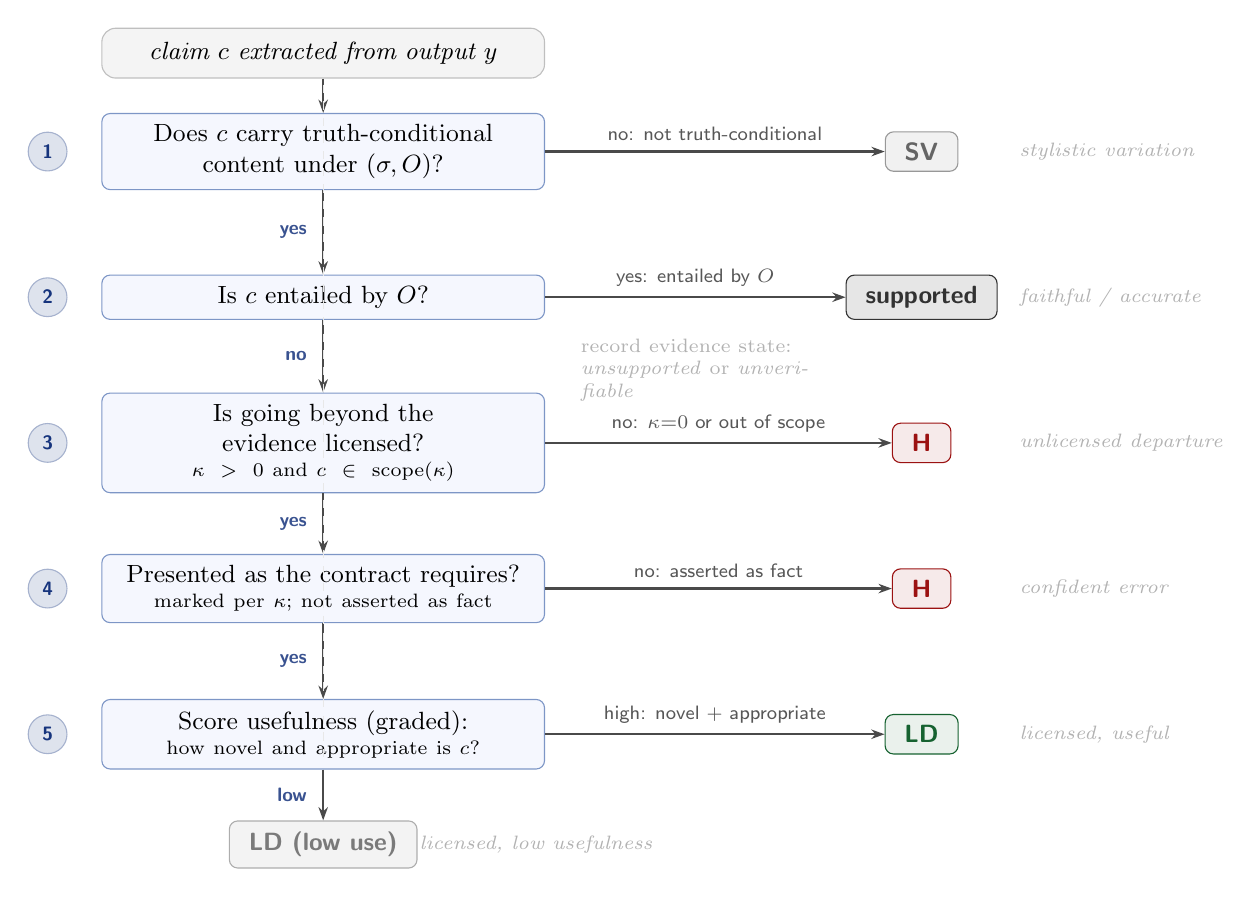
\begin{tikzpicture}[x=1cm, y=1cm]
\def\xS{0}\def\xE{7.6}\def\yS{-0.5}\def\dY{1.85}
\node[inpnode] (inp) at (\xS, 0.75) {claim $c$ extracted from output $y$};
\node[decnode] (t1) at (\xS, \yS) {Does $c$ carry truth-conditional content under $(\sigma, O)$?};
\node[decnode] (t2) at (\xS, \yS-\dY) {Is $c$ entailed by $O$?};
\node[decnode] (t3) at (\xS, \yS-2*\dY) {Is going beyond the evidence licensed?\\[-2pt]{\scriptsize $\kappa>0$ and $c\in\mathrm{scope}(\kappa)$}};
\node[decnode] (t4) at (\xS, \yS-3*\dY) {Presented as the contract requires?\\[-2pt]{\scriptsize marked per $\kappa$; not asserted as fact}};
\node[decnode] (t5) at (\xS, \yS-4*\dY) {Score usefulness (graded):\\[-2pt]{\scriptsize how novel and appropriate is $c$?}};
\node[lSV] (sv) at (\xE, \yS) {\textsf{SV}};
\node[lOK] (ok) at (\xE, \yS-\dY) {\textsf{supported}};
\node[lH]  (h1) at (\xE, \yS-2*\dY) {\textsf{H}};
\node[lH]  (h2) at (\xE, \yS-3*\dY) {\textsf{H}};
\node[lPD] (pd) at (\xE, \yS-4*\dY) {\textsf{LD}};
\node[lNE] (ne) at (\xS, \yS-4*\dY-1.4) {\textsf{LD} (low use)};
\draw[arr] (inp) -- (t1);
\draw[arr] (t1) -- node[spinelbl, left=4pt] {yes} (t2);
\draw[arr] (t2) -- node[spinelbl, left=4pt] {no}  (t3);
\draw[arr] (t3) -- node[spinelbl, left=4pt] {yes} (t4);
\draw[arr] (t4) -- node[spinelbl, left=4pt] {yes} (t5);
\draw[arr] (t5) -- node[spinelbl, left=4pt] {low}  (ne);
\draw[arr] (t1.east) -- node[exitlbl, above=2pt] {no: not truth-conditional} (sv.west);
\draw[arr] (t2.east) -- node[exitlbl, above=2pt] {yes: entailed by $O$} (ok.west);
\draw[arr] (t3.east) -- node[exitlbl, above=2pt] {no: $\kappa{=}0$ or out of scope} (h1.west);
\draw[arr] (t4.east) -- node[exitlbl, above=2pt] {no: asserted as fact} (h2.west);
\draw[arr] (t5.east) -- node[exitlbl, above=2pt] {high: novel + appropriate} (pd.west);
\node[annot, anchor=west] at (\xE+1.12, \yS) {stylistic variation};
\node[annot, anchor=west] at (\xE+1.12, \yS-\dY) {faithful / accurate};
\node[annot, anchor=west] at (\xE+1.12, \yS-2*\dY) {unlicensed departure};
\node[annot, anchor=west] at (\xE+1.12, \yS-3*\dY) {confident error};
\node[annot, anchor=west] at (\xE+1.12, \yS-4*\dY) {licensed, useful};
\node[annot, anchor=west] at (\xS+1.1, \yS-4*\dY-1.4) {licensed, low usefulness};
\node[annot, anchor=west, text width=3.0cm, align=left] at (3.15, {\yS-1.5*\dY}) {\emph{record evidence state:}\\ unsupported \emph{or} unverifiable};
\foreach \i/\yy in {1/\yS, 2/{\yS-\dY}, 3/{\yS-2*\dY}, 4/{\yS-3*\dY}, 5/{\yS-4*\dY}}
{\node[circle, fill=clrKw!14, draw=clrKw!38, font=\scriptsize\bfseries\sffamily, text=clrKw, inner sep=1.5pt, minimum size=1.4em] at (-3.5, \yy) {\i};}
\draw[gray!18, dashed, line width=0.4pt] (\xS, 0.35) -- (\xS, \yS-4*\dY-0.3);
\end{tikzpicture}}

\caption{\textbf{Claim-level annotation as a decision tree, for a contract $(O,\sigma,\kappa)$.}
\emph{Spine} (downward, blue labels): continue to the next test. \emph{Exit} (rightward, grey labels): immediate verdict.
The tree runs in three layers: an \emph{evidence state} (tests~1--2), a \emph{license and stance} check (tests~3--4), and a \emph{usefulness} score (test~5).
\textsf{SV}: stylistic variation (no truth-conditional content).
\textsf{supported}: entailed by $O$ (faithful/accurate).
A truth-conditional claim not entailed by $O$, whether \emph{unsupported} (contradicted or absent) or \emph{unverifiable} ($O$ holds no evidence either way), is not yet a verdict: its evidence state is recorded and it proceeds to the license check.
\textsf{H}: hallucination (test~3: an unlicensed departure, $\kappa{=}0$ or outside the licensed scope; test~4: a \emph{confident error}, asserted as verified fact where the license required a hedge or a declared frame).
\textsf{LD}: licensed divergence (licensed and presented as the contract requires); test~5 then scores its usefulness.
\textsf{LD} (low use): licensed divergence whose usefulness score is low.
Tests~1--2 can be assessed against $O$ (human annotation, or retrieval with natural language inference); test~3 is read from the $\kappa$ annotation; test~4 is a stance check on presentation; test~5 (usefulness) is a graded, evaluator-dependent \emph{soft label} (a score reported together with its disagreement, rather than collapsed into a single verdict) (Section~\ref{sec:agenda}).}
\label{fig:annotation-tree}
\end{figure*}

\paragraph{Worked example.}
Consider ``Explain photosynthesis in a poetic style, but keep the science accurate.''
Here the oracle is scientific world knowledge, $\sigma$ high because figurative language is requested, and $\kappa{=}0$ because the science must stay accurate.
Calling chlorophyll ``a green workshop for sunlight'' is stylistic variation, but claiming that plants make sugar from moonlight is \Hall.
If the prompt instead asks for a fictional plant ecology where moonlight powers growth, the same moonlight claim is \LD: clearly framed as invented and consistent with the fictional constraints.
Whether it enriches the fiction is evaluated separately.

\noindent Under this vocabulary we do not oppose ``creativity versus truth.''
We oppose \textbf{\Hall} (\TC\ violations) to \textbf{\LD} (\TC-compliant creativity); contract-blind factuality evaluation fails to separate the two.

% ============================================================
% Thesis-at-a-glance: example-driven summary of the framework
% ============================================================
\begin{table*}[t]
\centering
\small
\caption{\textbf{The thesis in one view.}
A fixed contract $\TC(p)=(O_p,\sigma_p,\kappa_p)$ sorts what an output adds into a violation (\Hall) or a licensed move (\LD, or merely stylistic), by what it licenses rather than by surface form.
$O$ is the oracle, $\sigma$ the form license, $\kappa$ the content license ($0$: none; $1$: flagged speculation; $2$: free invention).
Each card holds the contract fixed; across the cards, similar-looking claims receive different verdicts.
The brainstorming card shows an output-level verdict (too little licensed divergence, Section~\ref{sec:discussion}); the other verdicts are claim-level.}
\label{tab:thesis-at-a-glance}

\begin{tcolorbox}[regcard, colframe=cardStrict, colback=cardStrict!3, colbacktitle=cardStrict!13,
  borderline west={3.5pt}{0pt}{cardStrict},
  title={``Summarize this medical report''\hfill \skb{cardStrict}{$\sigma$ low}\,\skb{cardStrict}{$\kappa$ 0}}]
{\scriptsize\itshape Oracle $O$: the provided report.}\\[2pt]
\begin{tabularx}{\linewidth}{@{}>{\raggedright\arraybackslash}X c >{\raggedright\arraybackslash}p{4.1cm}@{}}
``the patient has diabetes'' (not in the report) & \bH & unsupported by $O$ \\
\end{tabularx}
\end{tcolorbox}

\begin{tcolorbox}[regcard, colframe=cardStyle, colback=cardStyle!3, colbacktitle=cardStyle!13,
  borderline west={3.5pt}{0pt}{cardStyle},
  title={``Explain photosynthesis like a poet, keep the science accurate''\hfill \skb{cardStyle}{$\sigma$ high}\,\skb{cardStyle}{$\kappa$ 0}}]
{\scriptsize\itshape Oracle $O$: scientific world knowledge.}\\[2pt]
\begin{tabularx}{\linewidth}{@{}>{\raggedright\arraybackslash}X c >{\raggedright\arraybackslash}p{4.1cm}@{}}
``chlorophyll, a green workshop for sunlight'' & \bNE & metaphor keeps the proposition intact \\
\addlinespace[2pt]
``plants make sugar from moonlight'' & \bH & new false claim; the form license does not cover it \\
\end{tabularx}
\end{tcolorbox}

\begin{tcolorbox}[regcard, colframe=cardFlag, colback=cardFlag!3, colbacktitle=cardFlag!13,
  borderline west={3.5pt}{0pt}{cardFlag},
  title={``List possible causes; flag anything unestablished''\hfill \skb{cardFlag}{$\sigma$ low}\,\skb{cardFlag}{$\kappa$ 1}}]
{\scriptsize\itshape Oracle $O$: world knowledge; flagged speculation licensed.}\\[2pt]
\begin{tabularx}{\linewidth}{@{}>{\raggedright\arraybackslash}X c >{\raggedright\arraybackslash}p{4.1cm}@{}}
``could be early Lyme disease, but speculative'' & \bPD & licensed speculation, marked as a hypothesis \\
\addlinespace[2pt]
``this is early Lyme disease'' (asserted) & \bH & confident error: asserted where a hedge (an explicit marker of uncertainty) was due \\
\end{tabularx}
\end{tcolorbox}

\begin{tcolorbox}[regcard, colframe=cardIdea, colback=cardIdea!4, colbacktitle=cardIdea!15,
  borderline west={3.5pt}{0pt}{cardIdea},
  title={``Write a short story set in 1920s Paris''\hfill \skb{cardIdea}{$\sigma$ high}\,\skb{cardIdea}{$\kappa$ 2}}]
{\scriptsize\itshape Oracle $O$: prompt constraints (declared fictional frame).}\\[2pt]
\begin{tabularx}{\linewidth}{@{}>{\raggedright\arraybackslash}X c >{\raggedright\arraybackslash}p{4.1cm}@{}}
invents a caf\'e and its owner & \bPD & invention inside the declared frame \\
\addlinespace[2pt]
a real figure asserts a quote they never made & \bH & real-world assertion outside the frame \\
\end{tabularx}
\end{tcolorbox}

\begin{tcolorbox}[regcard, colframe=cardIdea, colback=cardIdea!4, colbacktitle=cardIdea!15,
  borderline west={3.5pt}{0pt}{cardIdea},
  title={``Brainstorm ten product ideas''\hfill \skb{cardIdea}{$\sigma$ high}\,\skb{cardIdea}{$\kappa$ 2}}]
{\scriptsize\itshape Oracle $O$: prompt constraints; invention rewarded.}\\[2pt]
\begin{tabularx}{\linewidth}{@{}>{\raggedright\arraybackslash}X c >{\raggedright\arraybackslash}p{4.1cm}@{}}
only restates products that already exist & \bIP & too conservative for a contract that rewards invention \\
\end{tabularx}
\end{tcolorbox}

\begin{tcolorbox}[enhanced, colback=black!4, colframe=black!20, boxrule=0.35pt, arc=2pt,
  left=6pt, right=6pt, top=3pt, bottom=3pt, before skip=2pt, after skip=0pt]
\footnotesize\textbf{Reading rule.} A divergence is \bH\ or \bPD\ according to what the contract licenses, not the surface text; within a fixed contract the verdict still differs by what is licensed and how it is presented.
\end{tcolorbox}
\end{table*}

\paragraph{Why $\kappa$ is not reducible to faithfulness.}
Faithfulness asks whether an output stays within its evidence; $\kappa$ asks whether leaving it is licensed and, when it is, with what commitment the content must be presented.
The two differ at $\kappa{=}1$.
Consider a clinical triage prompt whose contract requests flagged speculation (``list possible causes, and mark anything not yet established'').
Two outputs carry the \emph{same} proposition.
One states it flatly, ``this is early Lyme disease''; the other qualifies it, ``this could be early Lyme disease, but it is speculative and needs serology.''
A faithfulness or factuality verifier scores the proposition, not its epistemic marking: against an oracle that cannot yet confirm the cause, both are unsupported, so both are flagged alike.
The contract separates them.
The flat assertion is a \Hall, a \emph{confident error} stated as fact where the license required a hedge, whereas the qualified version is \LD: licensed speculation, presented as the contract requires.
This is the \emph{faithful uncertainty} that \citet{yona_metacognition_2026} argue separates a trustworthy answer from a hallucinated one, aligning a claim's linguistic uncertainty with what the model actually knows.
The license $\kappa$ turns that alignment into an explicit, scored part of the contract. Faithfulness has no place for it. This is why no faithfulness metric can produce the verdict that $\kappa$ determines.

\paragraph{Scope and minimality of the contract.}
We claim $(O,\sigma,\kappa)$ is a \emph{sufficient} basis for the verdict (enough to flip, that is, reverse, the verdicts that current pipelines get wrong), rather than a complete model of everything evaluation must weigh.
One axis is deliberately left out: \emph{severity}.
A medical question and a trivia question can share an identical contract ($O=$ world knowledge, $\sigma$ low, $\kappa{=}0$), yet a fabricated drug dose and a wrong trivia date are not equally costly.
Severity differs, but the verdict does not: both fabrications are \Hall.
Severity therefore weights the penalty on a violation (Section~\ref{sec:agenda}); it does not decide whether a claim violates the contract, so it belongs to the scoring layer above $(O,\sigma,\kappa)$ rather than inside it.
Other plausible factors reduce to the three components instead of extending them: audience and genre act on evaluation through the oracle they select and the form license they grant.
For example, writing for children selects an age-appropriate oracle and a narrower form license; the verdict logic is unchanged.
We make no completeness claim.
$(O,\sigma,\kappa)$ is the smallest set that is already enough to correct the verdicts that current pipelines get wrong; adding components remains possible.

% ============================================================
% Truth contracts + divergences (conceptual table)
% ============================================================
% ============================================================
% Canonical contracts in the (sigma, kappa) plane
% ============================================================
\begin{figure*}[tb]
\centering
\resizebox{0.82\linewidth}{!}{%
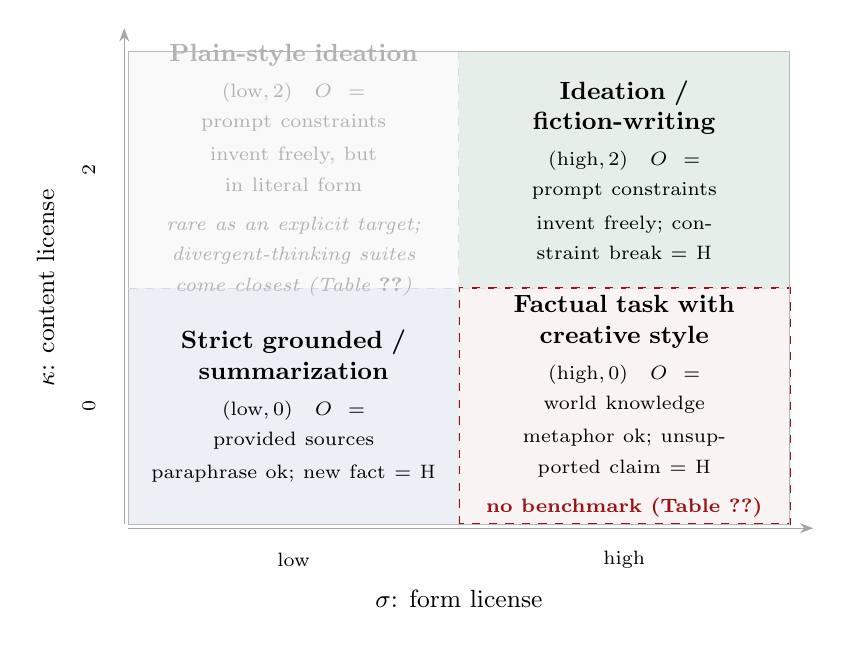
\begin{tikzpicture}[x=1cm,y=1cm,font=\small]
% quadrant fills (split at sigma=1 -> x=4.2, kappa=1 -> y=3)
\fill[clrKw!8]  (0,0) rectangle (4.2,3);
\fill[clrPD!11] (4.2,3) rectangle (8.4,6);
\fill[gray!5]   (0,3) rectangle (4.2,6);
\fill[clrH!5]   (4.2,0) rectangle (8.4,3);
\draw[clrH,thick,dashed] (4.2,0) rectangle (8.4,3);
\draw[gray!55] (0,0) rectangle (8.4,6);
\draw[gray!28,dashed] (4.2,0)--(4.2,6);
\draw[gray!28,dashed] (0,3)--(8.4,3);
% region content
\node[align=center, text width=3.8cm] at (2.1,1.5)
 {\textbf{Strict grounded /}\\\textbf{summarization}\\[2pt]
  {\scriptsize (low,\,$0$)\quad$O=$ provided sources}\\[1pt]
  {\scriptsize paraphrase ok; new fact $=$ \Hall}};
\node[align=center, text width=3.9cm] at (6.3,4.5)
 {\textbf{Ideation /}\\\textbf{fiction-writing}\\[2pt]
  {\scriptsize (high,\,$2$)\quad$O=$ prompt constraints}\\[1pt]
  {\scriptsize invent freely; constraint break $=$ \Hall}};
\node[align=center, text width=3.9cm] at (6.3,1.5)
 {\textbf{Factual task with}\\\textbf{creative style}\\[2pt]
  {\scriptsize (high,\,$0$)\quad$O=$ world knowledge}\\[1pt]
  {\scriptsize metaphor ok; unsupported claim $=$ \Hall}\\[3pt]
  {\scriptsize\bfseries\textcolor{clrH}{no benchmark (Table~\ref{tab:audit})}}};
\node[align=center, text width=3.9cm, text=gray!60] at (2.1,4.5)
 {\textbf{Plain-style ideation}\\[2pt]
  {\scriptsize (low,\,$2$)\quad$O=$ prompt constraints}\\[1pt]
  {\scriptsize invent freely, but in literal form}\\[3pt]
  {\scriptsize\itshape rare as an explicit target; divergent-thinking suites come closest (Table~\ref{tab:audit})}};
% axes
\draw[-{Stealth},gray!70] (0,-0.05)--(8.7,-0.05);
\draw[-{Stealth},gray!70] (-0.05,0)--(-0.05,6.3);
\node[font=\scriptsize] at (2.1,-0.45){low};
\node[font=\scriptsize] at (6.3,-0.45){high};
\node[font=\small] at (4.2,-0.95){$\sigma$: form license};
\node[font=\scriptsize,rotate=90] at (-0.5,1.5){$0$};
\node[font=\scriptsize,rotate=90] at (-0.5,4.5){$2$};
\node[font=\small,rotate=90] at (-1.05,3){$\kappa$: content license};
\end{tikzpicture}}
\caption{\textbf{Canonical truth contracts in the $(\sigma,\kappa)$ plane.}
$\sigma$ is form license (how freely form may vary), $\kappa$ the content license (whether new truth-conditional content may be introduced).
Each region names its oracle $O$, what divergence it allows, and what triggers a hallucination (\Hall).
Tinted regions are populated by existing benchmarks (Table~\ref{tab:audit}); the dashed region, a \emph{factual task with creative style}, is a canonical contract that no benchmark fills.
The fourth corner ($\sigma$ low, $\kappa{=}2$), plain-form invention, is rarely an explicit target (the divergent-thinking suites of Table~\ref{tab:audit} come closest); the important tension is in the dashed cell, where creative form meets a strict oracle.
The same surface divergence is acceptable or a violation according to the region, not the text \citep{maynez_faithfulness_2020,kryscinski_evaluating_2020,franceschelli_creativity_2024}.}
\label{fig:sk-map}
\end{figure*}

\subsection{Truth contracts and contract-relative divergence}\label{sec:truth-contracts}

The components of $\TC(p)=(O_p,\sigma_p,\kappa_p)$ combine into recognizable task profiles \citep{ji_survey_2023,huang_survey_2025}.
Figure~\ref{fig:sk-map} places the task profiles in the $(\sigma,\kappa)$ plane: three common contracts and one uncommon corner.
Existing benchmarks typically hold $O$ fixed but rarely annotate $(\sigma,\kappa)$ explicitly, making it easy to confuse \LD\ with \Hall\ \citep{bang_hallulens_2025}.

\paragraph{Claim-level labeling.}
Given a contract $\TC(p)$, each atomic claim is labeled \emph{stylistic variation} (form changes, no new propositions), \emph{supported} (entailed by $O$), \Hall\ (an unlicensed or mis-presented truth commitment), or \LD\ (licensed and presented as the contract requires, with usefulness scored separately) \citep{ji_survey_2023,bang_hallulens_2025}.
A minor truth-conditional inaccuracy is not a separate ``benign'' category but a low-severity \Hall, weighted in the scoring layer rather than excused (Section~\ref{sec:agenda}); a licensed divergence that adds little is still \LD, recorded with a low usefulness score rather than as a separate category.
\Hall\ and \LD\ are the two scored verdicts; the remaining labels are the non-divergent or negligible outcomes.

\noindent\textbf{Two-sided failure relative to $\kappa$.}
When $\kappa{=}0$, excess divergence increases \Hall; when $\kappa{>}0$, \emph{insufficient} divergence yields conservative outputs that fail the creative objective, a failure mode captured by creativity benchmarks but invisible to hallucination-only scoring \citep{hou_creativityprism_2025}.
The two sides sit at different levels: excess divergence is visible claim by claim, whereas insufficient divergence is an output-level absence, a distinction we make precise when defining verdicts (Section~\ref{sec:discussion}).
A contract-aware evaluator must therefore be able to fail an output in either direction, which a single unsupportedness count cannot.

With this vocabulary and labeling procedure in place, the natural question is whether existing benchmarks already condition their scores on the truth contract.
The next section examines both hallucination and creativity benchmarks and shows that they do not.

\section{The Diagnostic Gap: Evaluation That Ignores the Truth Contract}\label{sec:sota}

\paragraph{Two traditions, one shared blind spot.}
Hallucination benchmarks treat divergence from an oracle as a defect to minimize \citep{ji_survey_2023, bang_hallulens_2025}; creativity benchmarks treat it as evidence of novelty to maximize \citep{hou_creativityprism_2025}.
The split works for single-intent tasks but breaks down for mixed-intent prompts that pair novelty with factual constraints \citep{wang_user-centric_2024}: the same surface divergence can be \LD\ or \Hall, yet on both sides the truth contract $(O,\sigma,\kappa)$ stays implicit.
Table~\ref{tab:audit} documents the omission.
We conducted a purposive scoping audit of forty evaluation resources, organized by \emph{what} they evaluate (hallucination/faithfulness versus creativity/divergence) and by the \emph{task} they score.
In this sample, the pattern is uniform: the oracle $O$ is frequently fixed, but the form license $\sigma$ is never annotated and the content license $\kappa$ is never graded.
Hallucination benchmarks inherit a fixed $O$ and run at $\sigma$ low and $\kappa{=}0$ (neutral form, no invention); creativity benchmarks drop the factual oracle and run at $\kappa{=}2$, with $\sigma$ high in the writing suites; the few intent-aware benchmarks condition on the query without separating $\sigma$ from $\kappa$.
The contract is only implicit in the task label.

\paragraph{What the columns show, and what they do not.}
The $\sigma$ and $\kappa$ entries are \emph{our} annotations, inferred from each task's design rather than reported by the benchmark: a factual-QA or summarization suite implies $\sigma$ low and $\kappa{=}0$ (neutral form, no invention), a creative-writing suite implies $\sigma$ high and $\kappa{=}2$, and an open-ended innovation suite implies $\kappa{=}2$.
They are not measurements. What the audit documents is that no protocol scores these contract variables at all.
The point is not that the column entries repeat but that each one is inferred from the task, never scored: in this sample, no benchmark in either tradition turns the form license or the content license into a scored variable.

\paragraph{A missing evaluation setting.}
Annotated this way, the forty benchmarks cluster on a diagonal: hallucination suites at $\sigma$ low, $\kappa{=}0$ (neutral form, strict grounding) and creative-writing suites at $\sigma$ high, $\kappa{=}2$ (marked form, free invention).
The off-diagonal cell $\sigma$ high, $\kappa{=}0$ (vivid or figurative form under a strict factual contract) is filled by none of them, though Figure~\ref{fig:sk-map} marks it as a canonical contract (a factual task with creative style) and it names an everyday request (``explain this like a poet, but keep the science exact'').
That empty cell is not an accident: it is exactly where the form license and the content oracle conflict, and where an automatic verifier is most likely to misread marked form as unsupported content.
Worse, the only region where high $\sigma$ appears at all ($\sigma$ high, $\kappa{=}2$) is scored solely on creativity metrics, so no existing benchmark measures hallucination under high form license.
Building a benchmark for this cell (where creative form meets a strict oracle) is therefore a concrete priority of our agenda (Section~\ref{sec:agenda}).

\paragraph{How the audit was coded.}
We count a benchmark as annotating $\sigma$ only when form license is an explicit, scored variable in its protocol, not merely present in some prompts, and as grading $\kappa$ only when invention is a scored dimension with more than one licensed level.
By this criterion, \textsc{WritingBench} \citep{wu_writingbench_2025} is the most instructive case. It scores how well an output matches a requested \emph{style}, but it never treats the form license as a graded permission that conditions the truth measurement. By our test, $\sigma$ therefore stays unannotated, even though the task clearly implies a high $\sigma$.
The coding is a single-author pass against these criteria, offered as the first instance of the annotation layer we advocate rather than as a validated resource.
Borderline cases remain (does \textsc{WritingBench} \emph{score style} or \emph{annotate the form license}?), and independent re-coding with reported agreement is itself part of the agenda (Section~\ref{sec:agenda}).

\paragraph{An indicative observation.}
Preliminary observations of our own suggest that stylistic variation may affect measured hallucination rates.
However, our current pilot does not separate verifier sensitivity to form from genuine unsupported content, so we do not report it here.
We treat this observation only as motivation for the controlled, contract-aware study that our agenda specifies (Section~\ref{sec:agenda}).

\begin{table*}[!tp]
\centering
\scriptsize
\setlength{\tabcolsep}{4pt}
\renewcommand{\arraystretch}{0.95}
\caption{\textbf{Purposive scoping audit of forty evaluation resources against the truth-contract components $(O,\sigma,\kappa)$, grouped by what they evaluate and by task.}
For $\sigma$ and $\kappa$ we record \emph{our} annotation of the level each task implies ($\sigma$: form license; $\kappa$: content license); these are read from the task design, not reported or scored by any benchmark.
The audit tests whether the protocol scores these variables, not whether our annotations are independently measured data.
Legend: $\sigma$ as ``low''/``high'' and $\kappa$ as $0$/$1$/$2$ = the level the task implies but never makes an explicit, scored variable; ``--'' = not represented in the protocol.
In this sample, we found no protocol that explicitly conditions the hallucination verdict on the form or content license; oracle $O$ is the only component routinely fixed.
TTCT/TTCW: Torrance Tests of Creative Thinking/Writing; RAG: retrieval-augmented generation.}
\label{tab:audit}
\begin{tabular}{p{0.335\textwidth} p{0.135\textwidth} p{0.165\textwidth} c c p{0.155\textwidth}}
\toprule
\textbf{Benchmark} & \textbf{Task evaluated} & \textbf{Oracle $O$} & \boldmath$\sigma$ & \boldmath$\kappa$ & \textbf{Contract} \\
\midrule
\addlinespace[1pt]
\multicolumn{6}{l}{\textbf{Evaluates hallucination / faithfulness}} \\
\addlinespace[1pt]
FEVER \citep{thorne_fever_2018} & Fact-checking & Wikipedia evidence & low & $0$ &Implicit (strict) \\
TruthfulQA \citep{lin_truthfulqa_2022} & Factual QA & World knowledge & low & $0$ &Implicit (strict) \\
PopQA \citep{mallen_when_2023} & Long-tail QA & Wikidata & low & $0$ &Implicit (strict) \\
SimpleQA \citep{wei_measuring_2024} & Factual QA & World knowledge & low & $0$ &Implicit (strict) \\
TriviaQA \citep{joshi_triviaqa_2017} & Reading-comp.\ QA & Evidence documents & low & $0$ &Implicit (strict) \\
DefAn \citep{rahman_defan_2024} & Factual QA & World knowledge & low & $0$ &Implicit (strict) \\
HaluEval \citep{li_halueval_2023} & QA + summarization & World knowl.\ + ctx & low & $0$ &Implicit (strict) \\
FactBench \citep{bayat_factbench_2024} & Factual QA & World knowledge & low & $0$ &Implicit; \texttt{undecidable} \\
HalluLens \citep{bang_hallulens_2025} & Factual QA & World knowledge & low & $0$ &Implicit (strict) \\
FRANK \citep{pagnoni_understanding_2021} & Summarization & Source (news) & low & $0$ &Implicit (strict) \\
QAGS \citep{wang_asking_2020} & Summarization & Source (news) & low & $0$ &Implicit (strict) \\
SummEval \citep{fabbri_summeval_2021} & Summarization & Source (news) & low & $0$ &Implicit (strict) \\
XSum \citep{narayan_xsum_2018} & Summarization & Source (BBC) & low & $0$ &Implicit (strict) \\
CNN/DailyMail \citep{hermann_teaching_2015} & Summarization & Source (news) & low & $0$ &Implicit (strict) \\
DelusionQA \citep{sadat_delucionqa_2023} & Domain QA & Source (manuals) & low & $0$ &Implicit (strict) \\
HaluQA \citep{cheng_evaluating_2023} & Long-form QA & World knowledge & low & $0$ &Implicit (strict) \\
BIG-Bench \citep{srivastava_beyond_2023} & Multi-task reasoning & Task gold & low & $0$ &Implicit (strict) \\
BIG-Bench Hard \citep{suzgun_challenging_2023} & Reasoning & Task gold & low & $0$ &Implicit (strict) \\
CR-LLM \citep{li_cr-llm_2024} & Concept reasoning & Concept gold + ctx & low & $0$ &Implicit (strict) \\
HotpotQA \citep{yang_hotpotqa_2018} & Multi-hop QA & Wikipedia & low & $0$ &Implicit (strict) \\
HypoTermQA \citep{uluoglakci_hypotermqa_2024} & Hypothetical QA & World knowledge & low & $0$ &Implicit (strict) \\
HalluRAG \citep{ridder_hallurag_2025} & RAG QA & Retrieved Wikipedia & low & $0$ &Implicit (strict) \\
ToolQA \citep{zhuang_toolqa_2023} & Tool-use QA & Tools / APIs & low & $0$ &Implicit (strict) \\
RealTimeQA \citep{kasai_realtime_2024} & Real-time QA & Current events & low & $0$ &Implicit (strict) \\
FaithQA \citep{hao_faithqa_2025} & Intent verification & Query constraints & -- & -- & Partial; intent only \\
HIC-Bench \citep{yang_hicbench_2025} & Hallucination typing & Task-dependent & -- & $2$ &Partial; intel./defect. \\
\midrule
\addlinespace[2pt]
\multicolumn{6}{l}{\textbf{Evaluates creativity / divergence}} \\
\addlinespace[1pt]
CreativityPrism \citep{hou_creativityprism_2025} & Multi-task creativity & None (rubric) & high & $2$ &Absent \\
LitBench \citep{fein_litbench_2025} & Story evaluation & None (human pref.) & high & $2$ &Absent \\
Short Story \citep{ismayilzada_evaluating_2025} & Story generation & None (sem./human) & high & $2$ &Absent \\
WritingBench \citep{wu_writingbench_2025} & Creative writing & None (rubric/human) & high & $2$ &Absent \\
Art-or-Artifice / TTCW \citep{chakrabarty_art_2024} & Creative writing & None (expert rubric) & high & $2$ &Absent \\
Automated DT scoring \citep{organisciak_beyond_2023} & Divergent thinking & None (auto.\ scoring) & -- & $2$ &Absent \\
Verbal Creativity \citep{dinu_testing_2025} & Divergent thinking & None (TTCT) & -- & $2$ &Absent \\
Automated Creativity \citep{li_automated_2025} & Creative writing & Reference texts & high & $2$ &Absent \\
Hallu.\ Narratives \citep{sun_hallucinating_2024} & Controlled story & Mixed & high & $2$ &Absent; unlabeled \\
MacGyver \citep{tian_macgyver_2025} & Problem-solving & Feasibility (human) & -- & $2$ &Partial; correctness \\
EscapeBench \citep{qian_escapebench_2025} & Agent puzzles & Env.\ state (auto) & -- & $2$ &Partial; correctness \\
CreativEval \citep{delorenzo_creativeval_2024} & Code generation & Spec / correctness & -- & $2$ &Partial; correctness \\
NeoCoder \citep{lu_benchmarking_2025} & Code generation & Unit tests & -- & $2$ &Partial; correctness \\
Math Creativity \citep{ye_assessing_2024} & Math problem-solving & Soundness (human) & -- & $2$ &Partial; correctness \\
\bottomrule
\end{tabular}
\end{table*}

\subsection{Hallucination evaluation assumes a strict contract}
Hallucination evaluation is anchored in the choice of an oracle, either \emph{world knowledge} (\Acc: factuality) or \emph{provided context} (\Faith: faithfulness), with further axes for contradiction versus fabrication and evaluation granularity \citep{ji_survey_2023, bang_hallulens_2025}.
Modern protocols rely on claim-level decomposition and automated verification, for example, retrieval with natural language inference (NLI) \citep{chen_menli_2023} or QA-based checking \citep{wang_asking_2020}, building on fact-checking \citep{thorne_fever_2018}.
These pipelines are technically mature: atomic-claim decomposition is established \citep{min_factscore_2023}, joint decomposition and verification run at scale \citep{rajendhran_verifastscore_2025}, some verifiers add a third \texttt{undecidable} verdict \citep{bayat_factbench_2024}, and complementary signals such as semantic entropy \citep{farquhar_detecting_2024} or internal probes \citep{marks_geometry_2023} flag unsupported content without consulting any prompt-level contract.
Yet these axes are necessary, not sufficient, for contract-aware judgment: most pipelines assume a strict content license ($\kappa{=}0$), so any unsupported truth-conditional content is a failure.
The assumption is defensible in grounded generation but collapses when prompts license speculation, and even a three-way verdict with \texttt{undecidable} \citep{bayat_factbench_2024} refines the label space without consulting the contract: licensed invention is not merely undecidable --- the contract \emph{allows} it.

\subsection{Creativity evaluation leaves the oracle implicit}
Creativity is commonly defined as combining \emph{novelty} with \emph{value/appropriateness} under constraints \citep{runco_standard_2012}, but operationalizations vary sharply across tasks \citep{acar_creativity_2019, franceschelli_creativity_2024}.
Recent LLM work treats creativity as multi-dimensional, with benchmarks spanning divergent-thinking rubrics, creative-writing evaluation, and constrained problem solving; \textsc{CreativityPrism} typifies the trend by aligning heterogeneous tasks to shared quality, novelty, and diversity dimensions \citep{hou_creativityprism_2025, fein_litbench_2025}.
Such scores also remain evaluator-dependent: ratings shift with rubric design and rater background, changing model rankings even under identical prompts when using LLM-as-judge protocols \citep{ismayilzada_evaluating_2025, liu_g-eval_2023, zheng_judging_2023}.
From a \TC\ perspective, the deeper issue is that creativity benchmarks rarely treat the truth contract as an explicit variable: novelty can be rewarded without distinguishing \LD\ from \Hall\ \citep{sui_confabulation_2024, padmakumar_measuring_2025}, even when factual grounding is part of the contract \citep{wang_user-centric_2024}.
Faithfulness metrics could detect such violations \citep{maynez_faithfulness_2020, chen_menli_2023}, but they are not integrated into creativity pipelines.

\subsection{The shared failure mode and the closest prior work}
When $\TC$ is left implicit, two symmetric errors arise.
Under a permissive contract ($\kappa{>}0$), strict factuality checks misclassify licensed speculation as \Hall\ (false positives on \LD) \citep{cyriac_metrics_2025, sui_confabulation_2024}; under a strict contract ($\kappa{=}0$), novelty-oriented scores reward confident fabrications that inflate apparent originality (false negatives on \Hall) \citep{liu_g-eval_2023, chen_menli_2023}.
Uncertainty and abstention methods address the strict-contract case: when support is insufficient, a system should hedge, refuse, or defer rather than assert.
Our point is separate: under $\kappa{>}0$, the question is not only whether the model should abstain, but whether the prompt licenses a hedged or inventive move in the first place.
The closest existing steps narrow but do not close the gap.
Intent-hallucination evaluation decomposes a query into intent constraints (subject, action, qualifiers, quantity, and the like) and conditions the verdict on whether the response covers them \citep{hao_faithqa_2025}.
But it defines failure independently of factual accuracy and supplies no oracle.
It also treats flagged invention as a misinterpretation rather than a licensed move: it encodes neither $O$ nor $\kappa$.
A recent benchmark splits hallucinations into ``intelligent'' and ``defective,'' the closest analogue to the \LD/\Hall\ distinction \citep{yang_hicbench_2025}.
But it derives that label from the output's creativity and factual-deviation scores rather than from the prompt.
The label is therefore determined by the text and cannot flip with the contract that should govern it.
Closest in spirit, \citet{jiang_survey_2024} survey hallucination from a creativity perspective and ask whether hallucinated content can be creatively valuable.
We differ by shifting the unit of analysis: not the potential value of the content, but the prompt-level truth contract that decides whether unsupported content is licensed at all.
A domain-specific instance of the same tension appears in legal summarization. \citet{bendahman_hallucinations_2025} observe that expert reference summaries introduce legal entities that are absent from the source document, yet factual under domain knowledge. Their entity-guided system preserves these factual hallucinations while reducing the non-factual ones. In our terms, the status of such an entity turns on the oracle: a hallucination under $O=$ the source document alone, but supported once $O$ expands to the legal dataset and domain knowledge.
None of these makes $(O,\sigma,\kappa)$ a scored variable; that layer is what we argue for.

\subsection{Why universal suppression of \Hall\ is neither feasible nor desirable}
For sufficiently general generative models operating on open or incompletely observed distributions, perfect elimination of \Hall\ cannot be guaranteed.
Two independent formal arguments support this claim.
The first is statistical.
\citet{kalai_calibrated_2024} show that for calibrated language models, the probability of hallucinating an \emph{arbitrary} fact --- one whose truth value cannot be determined from the training corpus --- is bounded below by the fraction of facts that occur only once in training, a Good-Turing estimate of missing mass.
The bound holds even for ideal, error-free training data and does not depend on the Transformer architecture, though post-training can reduce it, typically at some cost to calibration.
Controlled experiments on n-gram and fine-tuned Transformer models confirm the predicted relationship between the rate of singly-occurring facts and the measured hallucination rate \citep{miao_hallucination_2025}.
The second argument is computability-theoretic: a computable model cannot learn every computable function, so a language model used as a general-purpose solver must answer incorrectly on some inputs \citep{xu_hallucination_2024}.
This is a worst-case result: it establishes that such inputs exist, not how often real users encounter them.
\citet{banerjee_llms_2024} reach a related conclusion from undecidability and G\"odel's incompleteness theorem, though their argument is broader and its extension to ordinary factual error is more contestable than the statistical bound above.

Neither argument implies a constant, irreducible error rate in deployment.
\citet{kalai_why_2025} trace much of the practical persistence of hallucination to training and evaluation incentives rather than to inevitability alone: when correct and incorrect statements are not perfectly separable, standard benchmarks score a confident guess above an honest abstention, so optimizing for benchmark performance optimizes for guessing.
\citet{suzuki_negligible_2025} show that logical inevitability and statistical negligibility can coexist: a model may still fail on an infinite set of inputs while the probability of encountering such a failure is pushed arbitrarily low with sufficient data quality and appropriate algorithms.
Empirically, strict contracts still show large residual error rates on short-form QA and truthfulness benchmarks \citep{mallen_when_2023, lin_truthfulqa_2022}, consistent with a floor that current methods have not closed.
The relevant mechanism is therefore not stochasticity alone but the interaction of incomplete data, generalization, calibration, and open-ended generation: a model must generalize beyond its observed corpus to remain useful, and assigning probability to unseen outputs creates some nonzero possibility of generating unsupported ones.

Alignment tuning adds to the problem rather than solving it. The refusal, hedging, and abstention policies learned during alignment tuning are themselves implicit contract commitments, chosen by the provider: they change the conditions under which a model refuses to diverge \citep{ouyang_training_2022}.
The same generative mechanism that produces unsupported claims also produces the novel hypotheses users request: \citet{sun_hallucinating_2024} formalize ``good hallucinations'' as reasoning paths that remain correct after convergence, and \citet{banerjee_does_2025} show that verification-style mitigation can preserve divergent thinking whereas some decoding interventions suppress it.
Because \Hall\ has a structural floor and the same divergence drives \LD, the practical goal is not universal suppression but contract-calibrated control: specify the contract, license divergence where the contract allows it, and require support before anything is presented as fact \citep{bang_hallulens_2025, he_shakespearean_2025}.

\section{Applying the Framework: Worked Verdicts}\label{sec:worked}

The audit shows that the contract is missing; this section shows that supplying it \emph{changes verdicts}.
We apply the decision rule of Section~\ref{sec:framework} by hand to four illustrative cases.
Cases~A--C each flip the verdict on the \emph{same} claim when one component of $(O,\sigma,\kappa)$ changes; Case~D is a scope boundary that does not flip.
Each instantiates a documented phenomenon: extrinsic-but-factual XSum hallucinations (A) \citep{maynez_faithfulness_2020}, fictional role-play (B and D) \citep{sadeq_mitigating_2024}, and FactBench's \texttt{undecidable} label (C) \citep{bayat_factbench_2024}.
Apart from Case~A, which cites a specific annotated XSum item, the claim strings are constructed test cases rather than verbatim dataset items; their role is to isolate a verdict that current pipelines cannot decide.
Table~\ref{tab:worked} summarizes the outcomes.

\paragraph{Case A: correct but unsupported (oracle shift).}
\citet{maynez_faithfulness_2020} document this pattern directly on XSum, where annotators label a summary span as an \emph{extrinsic but factual} hallucination: content not found in the source document yet factually correct.
A concrete annotated instance is XSum item \texttt{bbcid~28328378} (system \textsc{BERTS2S}), whose summary adds that the owners of a fire-destroyed recycling plant in Greater Manchester had been stripped of their environmental permit---content that the annotators mark as extrinsic (absent from the source article) yet unanimously judge factual.
Decomposing the output to the claim level isolates this added proposition as a single truth-conditional claim.
Under the summarization contract $O=$ the source, $\sigma$ low, $\kappa{=}0$, the claim is truth-conditional and unsupported by $O$: it is \Hall, even though it satisfies factuality (\Acc) against world knowledge.
If we keep the output fixed and change only the oracle (``What became of the plant's operators?'', with $O=$ world knowledge), the same claim becomes supported, so it is no longer \Hall.
This flip is exactly the unresolved question that Maynez et al.\ raise: should summaries tolerate such factual hallucinations \citep{maynez_faithfulness_2020, kryscinski_evaluating_2020}? The framework attributes it to $O$ rather than to the text.
Case~A is not specific to news summarization: \citet{bendahman_hallucinations_2025} document the same extrinsic-but-factual pattern at the entity level in legal summarization, where an entity absent from the source but certifiable against the legal record flips from \Hall\ to supported exactly as the oracle expands.

\paragraph{Case B: licensed invention that flips with the frame (license shift).}
Fictional role-play makes this routine \citep{sadeq_mitigating_2024}.
Take a single claim: that a certain café and its proprietor existed in 1920s Paris.
Under a historical-QA prompt ($O=$ world knowledge, $\kappa{=}0$), the café is unsupported and asserted as fact: it is \Hall.
Under ``write a short story set in 1920s Paris'' ($\kappa{=}2$), the \emph{same} invented café is a pretended assertion the frame licenses \citep{searle_logical_1975}: it is \LD, and how well it serves the story is its usefulness score.
Only the content license changed; the claim, and its surface form, did not change.
This is a flip that a novelty-oriented score and a factuality score each miss, from opposite sides \citep{hou_creativityprism_2025, sui_confabulation_2024}.

\paragraph{Case C: undecidable does not settle the verdict (license shift).}
FactBench's VERIFY pipeline labels each verifiable unit \texttt{supported}, \texttt{unsupported}, or \texttt{undecidable}, the last when retrieved evidence is insufficient to confirm or refute it, and its hallucination score penalizes \texttt{undecidable} units at a fixed weight regardless of what the prompt asked for \citep{bayat_factbench_2024}.
A FactBench-style instance is a model claim that a tool ``supports multiple input formats,'' which a verifier may mark \texttt{undecidable} when support varies across versions.
That label follows evidence availability, not the contract: under $\kappa{=}0$, asserting such a claim as established fact is \Hall\ and the penalty is warranted; under $\kappa{=}1$ (flagged speculation), the same epistemically undecidable content, marked as a hypothesis, is \LD.
The epistemic status (undecidable) is constant; the verdict is set by the license $\kappa$. A fixed penalty on undecidable content cannot capture this --- even a three-way verdict cannot.

\paragraph{Case D: a scope boundary that does not flip.}
Not every invention a fictional frame contains is licensed by it.
In the same 1920s-Paris story, suppose the model has a real, named historical figure assert a specific claim that figure never made, presented as biographical fact.
This is a genuine assertion about the real world, so it steps outside the declared frame: the claim falls outside the licensed scope ($c\notin\mathrm{scope}(\kappa)$) and stays \Hall\ even under $\kappa{=}2$ \citep{searle_logical_1975}.
Case~D shows the limit of $\kappa$: a license reaches only the content inside its declared scope, which is what separates the invented café of Case~B from a fabricated real-world fact placed beside it.

\begin{table}[htbp]
\centering
\small
\setlength{\tabcolsep}{3pt}
\renewcommand{\arraystretch}{1.2}
\caption{Worked verdicts. Cases~A--C flip the \emph{same} claim by changing one component of $(O,\sigma,\kappa)$: an oracle shift (A), a license shift (B), and a stance/license shift (C). Case~D is a scope boundary that does \emph{not} flip; the verdict follows the contract, not the surface text.}
\label{tab:worked}
\begin{tabular}{@{}p{0.06\columnwidth} p{0.29\columnwidth} p{0.28\columnwidth} p{0.29\columnwidth}@{}}
\toprule
\textbf{Case} & \textbf{Claim} & \textbf{Contract that yields \Hall} & \textbf{Contract that yields \LD\,/\,supported} \\
\midrule
A & extrinsic-but-factual claim, absent from source & $O=$ source, $\kappa{=}0$ & $O=$ world knowledge (supported) \\
B & an invented café in a 1920s-Paris story & historical-QA prompt, $\kappa{=}0$ & fiction prompt, $\kappa{=}2$ (\LD) \\
C & a possible cause, evidence undecidable & asserted as fact, $\kappa{=}0$ & flagged as hypothesis, $\kappa{=}1$ (\LD) \\
D & a fake quote by a real person & stated as biographical fact & stays \Hall\ even under $\kappa{=}2$ \\
\bottomrule
\end{tabular}
\end{table}

\noindent These verdicts are not measurements; they show that the rule is well-defined and that its output tracks the contract rather than the surface text.
That is the property current pipelines lack: a contract-blind scorer cannot justify the appropriate verdict in these cases without silently assuming a truth contract that it has no way to represent ($O$, $\sigma$, or $\kappa$).

\section{Research Agenda (Open Problems)}\label{sec:agenda}

If hallucination is contract-relative, evaluation must make the contract an explicit evaluation variable.
The framework and the audit lead to four research problems.
The first two concern measurement; the others concern benchmark and system design.
We present them as the paper's main forward contribution: not a finished evaluator, but the specification one would have to build.

\textbf{1. Contract annotation and inference.}
A contract-aware benchmark must annotate $O$, $\sigma$, and $\kappa$ independently rather than folding them into a task label.
The graded components are measurable today: the form license already has established datasets and metrics \citep{pavlick_empirical_2016, liu_semisupervised_2022}.
$\sigma$ could be turned into a graded scale: annotators compare pairs of outputs, and a comparative scoring model converts these judgments into scores; where its discrete levels should fall is a question for stylistic expertise that we leave open.
Users rarely state a formal contract, so $\TC(p)$ must also be inferred from prompt text \citep{wang_user-centric_2024, bodonhelyi_user_2024}.
Calibration is critical: misreading a strict prompt as permissive suppresses warranted penalties, and misreading a permissive prompt as strict penalizes legitimate \LD.
Contract inference must stay distinct from instruction-following fidelity: whether a model satisfied a verifiable format constraint is separately measurable \citep{zhou_ifeval_2023}, and an output can follow the requested form while violating $\kappa$.

\textbf{2. Reliable \Hall/\LD\ labeling.}
\LD\ is the framework's central new construct, and its two gates and usefulness score are not equally hard to obtain.
The licensing condition is read directly from the $\kappa$ annotation: under $\kappa{=}0$ no claim can be \LD, and under $\kappa{>}0$ one checks only whether the claim falls inside the licensed scope.
The stance condition is an explicitly checkable property of the text, close to the format constraints that instruction-following evaluation already scores \citep{zhou_ifeval_2023}.
The hard component is usefulness, the standard novelty-with-value criterion of creativity assessment \citep{runco_standard_2012, acar_creativity_2019, diedrich_are_2015}.
Novelty can be approximated automatically \citep{organisciak_beyond_2023}; value can be aggregated from pairwise preference judgments onto a continuous scale.
A practical \LD\ report therefore exposes three sublabels: license-pass, stance-pass, and a usefulness score (the predicates $L$ and $M$ and the score $U$ of Appendix~\ref{app:decision-rule}), with \LD\ assigned when the first two pass.
Because usefulness and contract boundaries are evaluator-dependent \citep{acar_creativity_2019, marco_reader_2025}, both should be reported as soft labels, with disagreement recorded rather than forced into consensus.
This is a proposed instrument, not a validated one; establishing its reliability is itself part of the agenda.

\textbf{3. Contract-aware benchmark design.}
No existing benchmark crosses task type, form license, and content license as independent variables; \textsc{CreativityPrism} and LitBench provide partial coverage but condition no scores on an explicit \TC\ \citep{hou_creativityprism_2025, fein_litbench_2025}.
Three needs follow.
First, metrics for \emph{excess} \Hall\ under a given contract: severity weighting, claim- versus output-level aggregation, and contract-conditioned baselines; severity-aware proposals exist \citep{bang_hallulens_2025, wei_measuring_2024}, but none conditions severity on an explicit contract.
Second, verifiers that are robust to stylistic variation: NLI-based verifiers risk treating figurative language as unsupported claims \citep{chen_menli_2023, aynetdinov_semscore_2024}, a fragility already visible in style-transfer metric meta-evaluations \citep{lai_multidimensional_2023, pauli_mind_2025}; a diagnostic suite pairing identical propositional content with varying styles \citep{jin_deep_2022} would separate verifier sensitivity to form from genuine divergence in content.
Third, a claim-level annotation layer (supported, hallucination, licensed divergence, unverifiable, stylistic variation), evaluated as a research object in its own right, including whether it changes model rankings or chiefly sharpens error diagnosis.
An emerging effort in this direction is CLEF~2026 SimpleText Task~2 (\emph{controlled creativity} in scientific text simplification): it targets grounded transformation ($\kappa{=}0$ with a granted form license: the form may change while new content must not be introduced) and annotates system outputs for overgeneration and information distortion, though it does not treat $(O,\sigma,\kappa)$ as jointly scored variables \citep{simpletext_task2_2026}.

\textbf{4. Mitigation that reduces \Hall\ while preserving \LD.}
Mitigation (constrained decoding, retrieval augmentation, post-hoc verification) typically targets \Hall\ reduction without measuring the loss of creative quality, and the trade-off is asymmetric: verification-style interventions can preserve divergent thinking while some decoding constraints suppress it \citep{banerjee_does_2025, sun_hallucinating_2024, he_shakespearean_2025}.
A contract-aware protocol should report \emph{both} \Hall\ reduction and \LD\ preservation under the same contract.

\section{Discussion}\label{sec:discussion}

\subsection{Implications for evaluation practice}
The practical consequence of contract-relative evaluation is a shift from defect counting to diagnosis conditioned on the truth contract.
Rather than asking ``how much does the output hallucinate?'', evaluation should ask ``does its divergence exceed what the \TC\ licenses?''
Three verdicts follow: \emph{aligned} (divergence matches the contract), \textit{excessive-}\textbf{\Hall} (unsupported claims where grounding is required), and \textit{insufficient-}\textbf{\LD} (output too conservative for a permissive contract).
The first two follow from the claim-level labels (a claim either is or is not \Hall); the third does not, because too little divergence is an \emph{absence} that no per-claim label can record.
\textit{Insufficient-}\LD\ is therefore an output-level judgment: it compares how much licensed divergence the output contains against what a permissive contract leads one to expect.
Creativity benchmarks already make this comparison when they penalize conservative outputs \citep{hou_creativityprism_2025}; the claim-level rule alone cannot deliver it.
The same measured rate therefore carries different meaning under strict and permissive contracts, so contract-specific baselines are not a refinement but a precondition for interpreting any score.
Even under permissive contracts, evaluation should still flag \emph{truth-commitment violations}, cases where invented content is presented as fact rather than as hypothesis or creative proposal \citep{bang_hallulens_2025, hou_creativityprism_2025}.

\subsection{Limitations of the position}
Our argument is conceptual, and five limitations bound it.
First, the framework is partly \emph{normative}.
Deciding what $O$ ought to be, and what a contract \emph{should} ground, is a value judgment about a task, not a measurement that we can make from the text alone.
Reasonable annotators will therefore disagree on contract boundaries, and that disagreement will concentrate where the scope of $\kappa$ must be drawn (the frontier that Case~D illustrates).
The framework treats that disagreement as signal, not noise. Where annotators diverge on a contract boundary, the divergence is recorded as a soft label instead of being forced into a single verdict (Section~\ref{sec:agenda}). The normative choice then stays visible and auditable, instead of hiding inside an unstated default.
Second, $\TC(p)$ is an idealization, and an ambiguous prompt may not determine it fully; locating the contract at the prompt is a modeling choice, and inferring it reliably is an open problem (Section~\ref{sec:agenda}), not a solved preprocessing step.
Third, \LD\ is specified and we sketch a scoring protocol for it (Section~\ref{sec:agenda}), but we do not validate that protocol.
Its usefulness condition inherits the evaluator dependence of creativity assessment.
What we offer is a labeling rule and a measurement proposal, not a validated method for measuring \LD\ reliably at scale.
Fourth, we argue this position rather than establishing it with a controlled study.
The audit and worked verdicts show that the gap is real and that supplying $(O,\sigma,\kappa)$ resolves verdicts; they do not measure its prevalence.
Quantifying how much contract annotation changes evaluation outcomes at scale is left to future empirical work.
Fifth, the framework is single-turn: it locates the contract in one prompt $p$ and does not model how a truth contract is established or revised across the turns of a dialogue, a restriction we leave for future work.

\section{Conclusion}\label{sec:conclusion}

Hallucination is not a context-free property of a claim but a verdict relative to the prompt's truth contract.
The vocabulary introduced here, $\TC(p)=(O_p,\sigma_p,\kappa_p)$ together with \LD\ and \Hall, makes explicit what current hallucination and creativity evaluations leave implicit: which oracle defines the standard of support, how much form license is granted, and whether new truth-conditional content is licensed.
In our scoping audit, no benchmark encodes this contract, and applying the labeling rule by hand shows that supplying the contract flips verdicts that otherwise depend on which protocol happens to be used.
The agenda is therefore to move evaluation from defect counting to diagnosis conditioned on the truth contract, so that it can penalize harmful fabrication under strict contracts while preserving licensed divergence where exploration is the point.
The remaining work is to build the contract into benchmarks, and to measure how much it changes our conclusions about models. The first step, however, is simpler: stop scoring divergence as if every prompt asked for the same thing.

\appendix
\renewcommand{\thesection}{\Alph{section}}
\renewcommand{\thesubsection}{\Alph{section}.\arabic{subsection}}
\renewcommand{\thesubsubsection}{\Alph{section}.\arabic{subsection}.\arabic{subsubsection}}
\renewcommand{\theHsection}{appendix.\Alph{section}}
\renewcommand{\theHsubsection}{appendix.\Alph{section}.\arabic{subsection}}
\renewcommand{\theHfigure}{appendix.\Alph{section}.\arabic{figure}}
\renewcommand{\theHtable}{appendix.\Alph{section}.\arabic{table}}
\renewcommand{\theHequation}{appendix.\Alph{section}.\arabic{equation}}

\appendixsection{Formal Claim-Level Decision Rule}\label{app:decision-rule}
\noindent\textbf{Input:} a prompt $p$, an output $y$, and an oracle $O$.\\
\noindent\textbf{Output:} a label for every atomic claim in $y$.

\begin{enumerate}
    \item \textbf{Specify the contract.} Infer or state $\TC(p)=(O_p,\sigma_p,\kappa_p)$: what is truth-conditional, what is evidence-bound, what is optionally speculative, and what (if anything) may be invented.
    \item \textbf{Decompose.} Split $y$ into atomic claims, ideally at claim-level granularity.
    \item \textbf{Record the evidence state} of each truth-conditional claim $c$ against $O$: \emph{supported} (entailed), \emph{unsupported} (contradicted or absent), or \emph{unverifiable} ($O$ holds no evidence either way).
    \item \textbf{Label each claim $c$:}
    \begin{itemize}
        \item[supported] if $c$ is entailed by $O$; a non-truth-conditional claim is \emph{neither} (stylistic variation);
        \item[\Hall] if $c$ is unsupported or unverifiable \emph{and} its departure is unlicensed ($\kappa{=}0$ or $c\notin\mathrm{scope}(\kappa)$), or is asserted as verified fact where $\kappa$ required a hedge or a declared frame;
        \item[\LD] if the departure is licensed ($\kappa>0$ and $c\in\mathrm{scope}(\kappa)$) and presented as the contract requires; its usefulness is then scored separately, and a low score is recorded as such rather than as a separate category.
    \end{itemize}
\end{enumerate}
\noindent Figure~\ref{fig:annotation-tree} renders this rule as a decision tree. The evidence state (supported / unsupported / unverifiable) is recorded but does not by itself determine the verdict: an unverifiable claim is \Hall\ under $\kappa{=}0$ if asserted as fact, yet \LD\ under $\kappa{=}1$ if marked as a hypothesis (Case~C, Section~\ref{sec:worked}).
The supporting evidence for each step is given where the rule is introduced in Section~\ref{sec:framework}.

\paragraph{Formal statement.}
After separating purely stylistic variation using $\sigma_p$, define three predicates for each truth-conditional claim $c$ under a contract $\TC(p)=(O_p,\sigma_p,\kappa_p)$.
Each predicate matches one check of the rule above: $S$ is the evidence state, $L$ is \emph{license-pass}, and $M$ is \emph{stance-pass} (Section~\ref{sec:framework}).
\begin{align*}
S(c,O_p)&=
\begin{cases}
1 & \text{if } c \text{ is supported by } O_p,\\
0 & \text{otherwise;}
\end{cases}\\
L(c,\kappa_p)&=
\begin{cases}
1 & \text{if } \kappa_p>0 \text{ and } c\in\mathrm{scope}(\kappa_p),\\
0 & \text{otherwise;}
\end{cases}\\
M(c,\kappa_p)&=
\begin{cases}
1 & \text{if } c \text{ is presented with the stance } \kappa_p \text{ requires},\\
0 & \text{otherwise.}
\end{cases}
\end{align*}
The verdict is then
\[
V(c\mid p)=
\begin{cases}
\mathrm{SUP} & \text{if } S(c,O_p)=1,\\[1mm]
\LD & \text{if } S(c,O_p)=0 \,\land\, L(c,\kappa_p)=1 \,\land\, M(c,\kappa_p)=1,\\[1mm]
\Hall & \text{if } S(c,O_p)=0 \,\land\, \bigl(L(c,\kappa_p)=0 \,\lor\, M(c,\kappa_p)=0\bigr),
\end{cases}
\]
where $\mathrm{SUP}$ is the \emph{supported} label of Figure~\ref{fig:annotation-tree}.
Usefulness stays outside the verdict as a separate score $U(c,p)\in[0,1]$ reported over \LD\ claims.
The central thesis is the existence of contract-dependent verdicts:
\[
\exists\, c,\, p_1,\, p_2:\quad V(c\mid p_1)=\Hall \quad\land\quad V(c\mid p_2)=\LD.
\]
In prose: the same claim can be a hallucination under one contract and licensed divergence under another.



\bibliography{references}

\end{document}
